\documentclass[tikz,border=3pt]{standalone}
\usepackage[utf8]{inputenc}
\usepackage[T1]{fontenc}
\usepackage{lmodern}
\renewcommand{\familydefault}{\sfdefault}
\usepackage{sansmath}\sansmath
\usepackage{chemfig}
\usepackage{pgfplots}\pgfplotsset{compat=1.18,/pgf/number format/use comma,/pgf/number format/1000 sep={.}}
\usetikzlibrary{arrows.meta,calc,positioning,decorations.pathmorphing,patterns}
% paleta del sitio
\definecolor{nar}{HTML}{E8680C}\definecolor{narc}{HTML}{FFB35C}\definecolor{hielo}{HTML}{FFF3E8}
\definecolor{tinta}{HTML}{1D1D1F}\definecolor{gris}{HTML}{6E6E73}\definecolor{lila}{HTML}{7C5CF0}
\definecolor{azul}{HTML}{2F6FD6}\definecolor{menta}{HTML}{17A673}\definecolor{coral}{HTML}{E8342A}
\newcommand{\matraz}[3]{%
  \begin{scope}[shift={(#1,0)},scale=#2]
  \path[fill=#3] (-0.15,1.85) -- (-0.15,1.2) to[out=-90,in=90] (-0.75,0.5) to[out=-90,in=180] (-0.4,0) -- (0.4,0)
     to[out=0,in=-90] (0.75,0.5) to[out=90,in=-90] (0.15,1.2) -- (0.15,1.85) -- cycle;
  \draw[tinta,thick] (-0.15,2.5) -- (-0.15,1.2) to[out=-90,in=90] (-0.75,0.5) to[out=-90,in=180] (-0.4,0) -- (0.4,0)
     to[out=0,in=-90] (0.75,0.5) to[out=90,in=-90] (0.15,1.2) -- (0.15,2.5);
  \draw[tinta] (-0.22,1.85) -- (0.22,1.85);
  \end{scope}}
\begin{document}
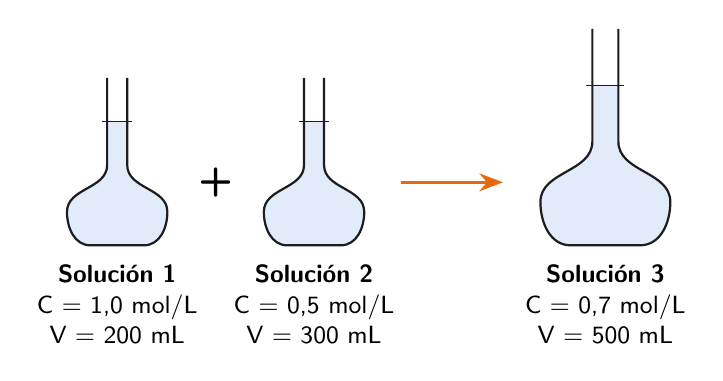
\begin{tikzpicture}[font=\small]
\matraz{0}{0.85}{azul!14}
\node[font=\Large\bfseries] at (1.25,0.8) {+};
\matraz{2.5}{0.85}{azul!14}
\draw[-{Stealth[length=3mm]},very thick,nar] (3.6,0.8) -- (4.9,0.8);
\matraz{6.2}{1.1}{azul!14}
\node[align=center] at (0,-0.75) {\textbf{Solución 1}\\C = 1,0 mol/L\\V = 200 mL};
\node[align=center] at (2.5,-0.75) {\textbf{Solución 2}\\C = 0,5 mol/L\\V = 300 mL};
\node[align=center] at (6.2,-0.75) {\textbf{Solución 3}\\C = 0,7 mol/L\\V = 500 mL};
\end{tikzpicture}
\end{document}
